\documentclass[12pt, oneside, a4paper]{book}
%\documentclass[12pt, a4paper]{book}
%----- 定義使用的 packages ----------------------

\usepackage{fontspec} 										% Font selection for XeLaTeX; see fontspec.pdf for documentation. 
\usepackage{xeCJK}											% 中文使用 XeCJK,但利用 \setCJKmainfont 定義粗體與斜體的字型
\defaultfontfeatures{Mapping=tex-text} 				% to support TeX conventions like ``---''
\usepackage{xunicode} 										% Unicode support for LaTeX character names (accents, European chars, etc)
\usepackage{xltxtra} 											% Extra customizations for XeLaTeX
\usepackage[sf,small]{titlesec}
\usepackage{amsmath, amssymb}
\usepackage{amsthm}										% theroemstyle 需要使用的套件
\usepackage{bm}                                                 % 排版粗體數學符號
\usepackage{enumerate}
\usepackage{graphicx, subfig, float} 					% support the \includegraphics command and options
\usepackage{array}
\usepackage{color, xcolor}
\usepackage{longtable, lscape}                                   % 跨頁的超長表格;lscape是旋轉此類表格的
\usepackage{threeparttable}                                     % 巨集,使表格加註解更容易(手冊p169)
\usepackage{multirow, booktabs}                                   % 讓表格編起來更美的套件(手冊p166),編輯跨列標題重覆的表格(手冊p182)
\usepackage{colortbl}                          				%.............................................表格標題註解之巨集套件
\usepackage{natbib}											% for Reference
\usepackage{makeidx}										% for Indexing
\usepackage[parfill]{parskip} % Activate to begin paragraphs with an empty line rather than an indent
%\usepackage{geometry} % See geometry.pdf to learn the layout options. There are lots.
%\usepackage[left=1.5in,right=1in,top=1in,bottom=1in]{geometry} 
\usepackage{url}                                                % 文稿內徵引網址
    \def\UrlFont{\rm}                                           % 網頁
\usepackage{fancyhdr}
	\pagestyle{fancy}
	\fancyhf{}                                     % 清除所有頁眉頁足
	\renewcommand{\headrulewidth}{0pt}                              % 頁眉下方的橫線    
%-----------------------------------------------------------------------------------------------------------------------
%  主字型設定
\setCJKmainfont
	[
		BoldFont=Heiti TC Medium								% 定義粗體的字型(依使用的電腦安裝的字型而定)
	]
	{cwTeX Q Ming Medium} 										% 設定中文內文字型
%	{新細明體}	
\setmainfont{Times New Roman}								% 設定英文內文字型
\setsansfont{Arial}														% used with {\sffamily ...}
%\setsansfont[Scale=MatchLowercase,Mapping=tex-text]{Gill Sans}
\setmonofont{Courier New}										% used with {\ttfamily ...}
%\setmonofont[Scale=MatchLowercase]{Andale Mono}
% 其他字型(隨使用的電腦安裝的字型不同,用註解的方式調整(打開或關閉))
% 英文字型
\newfontfamily{\E}{Cambria}										% 套用在內文中所有的英文字母
\newfontfamily{\A}{Arial}
\newfontfamily{\C}[Scale=0.9]{Cambria}
\newfontfamily{\T}{Times New Roman}
\newfontfamily{\TT}[Scale=0.8]{Times New Roman}
% 中文字型
\newCJKfontfamily{\MB}{微軟正黑體}							% 適用在 Mac 與 Win
\newCJKfontfamily{\SM}[Scale=0.8]{新細明體}				% 縮小版
%\newCJKfontfamily{\K}{標楷體}                        			% Windows 下的標楷體
\newCJKfontfamily{\K}{Kaiti TC Regular}         			% Mac OS 下的標楷體
\newCJKfontfamily{\BM}{Heiti TC Medium}					% Mac OS 下的黑體(粗體)
\newCJKfontfamily{\SR}{Songti TC Regular}				% Mac OS 下的宋體
\newCJKfontfamily{\SB}{Songti TC Bold}					% Mac OS 下的宋體(粗體)
\newCJKfontfamily{\CF}{cwTeX Q Fangsong Medium}	% CwTex 仿宋體
\newCJKfontfamily{\CB}{cwTeX Q Hei Bold}				% CwTex 粗黑體
\newCJKfontfamily{\CK}{cwTeX Q Kai Medium}   		% CwTex 楷體
\newCJKfontfamily{\CM}{cwTeX Q Ming Medium}		% CwTex 明體
\newCJKfontfamily{\CR}{cwTeX Q Yuan Medium}		% CwTex 圓體
%-----------------------------------------------------------------------------------------------------------------------
\XeTeXlinebreaklocale "zh"                  				%這兩行一定要加,中文才能自動換行
\XeTeXlinebreakskip = 0pt plus 1pt     %這兩行一定要加,中文才能自動換行
%-----------------------------------------------------------------------------------------------------------------------
%----- 重新定義的指令 ---------------------------
\newcommand{\cw}{\texttt{cw}\kern-.6pt\TeX}	% 這是 cwTex 的 logo 文字
\newcommand{\imgdir}{graph/}							% 設定圖檔的位置
\renewcommand{\tablename}{表}						% 改變表格標號文字為中文的「表」(預設為 Table)
\renewcommand{\figurename}{圖}						% 改變圖片標號文字為中文的「圖」(預設為 Figure)
\renewcommand{\contentsname}{目~錄}
\renewcommand\listfigurename{圖目錄}
\renewcommand\listtablename{表目錄}
\renewcommand{\appendixname}{附~錄}                  
\renewcommand{\indexname}{索引}
\renewcommand{\bibname}{參考文獻}
%-----------------------------------------------------------------------------------------------------------------------

\theoremstyle{plain}
\newtheorem{de}{Definition}[section]				%definition獨立編號
\newtheorem{thm}{定理}[section]			%theorem 獨立編號,取中文名稱並給予不同字型
\newtheorem{lemma}[thm]{引理}				%lemma 與 theorem 共用編號
\newtheorem{ex}{{\E Example}}						%example 獨立編號,不編入小節數字,走流水號。也換個字型。
\newtheorem{cor}{Corollary}[section]				%not used here
\newtheorem{exercise}{EXERCISE}					%not used here
\newtheorem{re}{\emph{Result}}[section]		%not used here
\newtheorem{axiom}{AXIOM}							%not used here
\renewcommand{\proofname}{\textbf{Proof}}		%not used here

\newcommand{\loflabel}{圖} % 圖目錄出現 圖 x.x 的「圖」字
\newcommand{\lotlabel}{表}  % 表目錄出現 表 x.x 的「表」字

\parindent=0pt

%--- 其他定義 ----------------------------------
% 定義章節標題的字型、大小
\titleformat{\chapter}[display]{\raggedleft\LARGE\bfseries\CF}		% 定義章抬頭靠右(\reggedleft)
 { 第\ \thechapter\ 章}{0.2cm}{}
%\titleformat{\chapter}[hang]{\centering\LARGE\sf}{\MB 第~\thesection~章}{0.2cm}{}%控制章的字體
%\titleformat{\section}[hang]{\Large\sf}{\MB 第~\thesection~節}{0.2cm}{}%控制章的字體
%\titleformat{\subsection}[hang]{\centering\Large\sf}{\MB 第~\thesubsection~節}{0.2cm}{}%控制節的字體
%\titleformat*{\section}{\normalfont\Large\bfseries\MB}
%\titleformat*{\subsection}{\normalfont\large\bfseries\MB}
%\titleformat*{\subsubsection}{\normalfont\large\bfseries\MB}


% 顏色定義
\definecolor{heavy}{gray}{.9}								% 0.9深淺度之灰色
\definecolor{light}{gray}{.8}
\definecolor{pink}{rgb}{0.99,0.91,0.95}               % 定義pink顏色
  

\title{ \LaTeX{\UD 表格應用}}
\author{{\NC 張馨云}\;\; {\JF 410578046}}
\date{{\BR \today}} 	

\begin{document}
\maketitle
\fontsize{12}{22 pt}\selectfont

\centerline{{\BCF 引言}}
\setlength{\parindent}{2em}   
	若設計得當,表格可使讀者更迅速且正確的掌握筆者所傳遞的資料信息。若表格過於繁複,可能會喪失其表達資訊的功能,故而表格排版應當簡單俐落。與WORD相比,\LaTeX 對表格的編排顯得更為專業:所有的表格編輯皆透過數據及指令表達,避免了手動排版的可能產生的表格錯誤與參差不齊。本文將介紹各式\LaTeX 表格的表示方法。
\bigskip
\section{{\BM 表格表示法}}
\subsection{\BM tabbling}
	tabbling完全使用空間、位置的配置來顯示表格內容,無線條指令來區隔,不見得一定要用於表格的排版,亦可用於表示條列。tabbing在\LaTeX 之中並非最小單位,故而不以最小單位的 box 處理,其製成的表格是可以跨頁的。因此,要和其他文字、圖表並排排版時,得另外放進一個 box 中,讓他自成一個 box 單位,例如 $\backslash$parbox 或 minipage 環境之中。 \\
	\indent 在 tabbing 環境中,第一個列(row)是以 「$\backslash$=」來標示 Tab 寬度來區隔欄位,
這個寬度是由欄位裡頭的字串寬度所決定的。後續的每個欄位則是由 「$\backslash$>」來區隔,
每列尾要自行加上 $\backslash\backslash$來換行,最後一行可以不必使用 $\backslash\backslash$ 換行。\\
tabbing 的基本結構為: \\
$\backslash$begin $\{$tabbing$\}$ \\
column1 \;$\backslash$=  column2 \;$\backslash$= \;column3 \;$\backslash\backslash$ \\
item1 \;$\backslash$> \;item2 \;$\backslash$> \;item3 \;$\backslash\backslash$ \\
itemA \;$\backslash$> \;itemB \;$\backslash$> \;itemC \\
$\backslash$end $\{$tabbing$\}$ \\
若想調整欄位寬度時可以使用 template 的方式,例如: \\
$\backslash$begin $\{$tabbing$\}$ \\
xxxxxxxxxx \;$\backslash$=  xxxxxxxxxx \;$\backslash$= \;xxxxxxxxxx \;$\backslash$kill \\
column1 \;$\backslash$=>  column2 \;$\backslash$> \;column3 \;$\backslash\backslash$ \\
item1 \;$\backslash$> \;item2 \;$\backslash$> \;item3 \;$\backslash\backslash$ \\
itemA \;$\backslash$> \;itemB \;$\backslash$> \;itemC \\
$\backslash$end $\{$tabbing$\}$ \\
	\indent 此處,10個x為欄位的寬度,$\backslash$kill 表示此行不print出來,且會自動換行。亦可使用表格中最長字串來表示欄位寬度,或是使用$\backslash$hspace$\{$6em$\}$ 等長度指令來設定欄位寬度。\\
練習:
\begin{tabbing}
\hspace{8em} \= \hspace{6em} \kill
姓名 \> 白小狼 \\
身分證字號 \> A123456789 \\
電子郵件信箱 \> whitewolf@gmail.com  \\
\end{tabbing}

\subsection{\BM tabular}
	和tabbling不同的是,tabular具有框線,並且\LaTeX 把整個表格當作一個單位來處理,版面的安排與一般字母無異。分隔欄位的符號為$\&$,並且必須指定表格欄內文字的置放位置,超出指定欄位寬度時,會自動換行。

\subsubsection{\BM tabular的基本語法}
\noindent 以tabular表示最基本的表格形式: \\
$\backslash$begin $\{$tabular$\}$[t]$\{$ccc$\}$
$\backslash$hline \\
column1 \;$\&$ \;column2 \;$\&$ \;column3 \;$\backslash\backslash$  \\
$\backslash$hline \\
item1 \;$\&$ \;item2 \;$\&$ \;item3 \;$\backslash\backslash$\\
itemA \;$\&$ \;itemB \;$\&$ \;itemC \;$\backslash\backslash$\\
$\backslash$hline \\
$\backslash$end $\{$tabular$\}$

	\indent 其中,$\&$表示下一行;[t或b或c]設置位置,t為top,b表示bottom,而c表示center。\LaTeX 會把整個tabular表格當成一個字母單位,故而可以與其他文字、圖表並排排版。這些參數在當前後有文字並排時才會顯其作用,表示和同行文字的對其方式,top 是表格頂端和前後文字對齊,bottom 則是表格底部和前後文字對齊,center 則是和表格中央對齊。換行的方式和 tabbing 相同,其中,$\backslash$hline是畫一條水平框線的意思,$\backslash$hline$\backslash$hline則會畫雙線,$\backslash$hline之後不須加$\backslash\backslash$來換行。$\{$ccc$\}$則表示個欄位內容在方框內的置放位置,l表示left,靠左;r表示right,靠右;c表示center,置中。若需要在表格中加上垂直光線時,則在表示位置的地方加上「|」,例如:$\{$|c|c|c|$\}$,加入「||」則會畫雙縱線。


\subsubsection{\BM tabular對欄位的調整}\label{option_col}
\begin{enumerate}[a. ]
	\item \textbf{p$\{$寬度$\}$}:此處的p指的是段落(paragraph)。通常指定了寬度後段落中的文字會自動折行,且此段落的頂端會和其他欄位的頂端對齊。
	\item \textbf{@$\{$文字、符號或指令$\}$}:可作用在各列,使其出現某個文字、符號,或都在某個指令的作用下。同時,此指令會將欄為間距縮為0。若置於首尾,有使水平線與文字切齊的作用。
	\item \textbf{$\backslash$multicolumn$\{$欄位數$\}\{$左右位置$\}\{$文字內容$\}$}:跨欄排版。如一段文字跨兩欄。左右位置可使用 lrc 之一。
	\item \textbf{$\backslash$cline$\{$a-b$\}$}:畫某部分欄位的水平線。其中a與b表示要畫線的欄位數。如:$\backslash$cline$\{$3-4$\}$即為畫第二欄至第三欄的水平線。
	\item \textbf{$\backslash$arrayrulewidth=單位長度}:調整表格線條的粗細,預設為0.4pt,置於tabular起始之前。
	\item \textbf{$\backslash$tabcolsep=單位長度}:調整兩欄位的左右間距,預設為6pt。此值為實際兩欄位間距值的一半,置於tabular起始之前。
	\item \textbf{$\backslash$doublerulesep=單位長度}:調整畫雙線時,這兩線間的間距,預設值是 2pt,置於tabular起始之前。
	\item 以不同物質的比熱為例,製作表\ref{ex_SpecHeat}:
 		\begin{tabbing}
 		\hspace{18em} \= \hspace{6em} \kill
 		$\backslash$renewcommand$\{\backslash$arraystretch$\}\{$1.2$\}$ \> 加大表格間距為原來的1.2倍 \\
 		$\backslash$arrayrulewidth=1pt  \> 調整線條粗細為 1pt \\
 		$\backslash$tabcolsep=12pt \> 調整欄間距為 24pt \\
 		$\backslash$begin$\{$tabular$\}\{$@$\{\backslash$ HC $\}$l l l@$\{  \} \}$ \> 第一欄位使用「華康兒風體W4」字族 \\
 		$\backslash$multicolumn$\{$2$\}\{$c$\}\{\backslash$bf Specific Heats\} \>  跨2欄排版,文字置中 \\
 		$\backslash$cline$\{$2-3$\}$ \> 只畫二三欄水平線,分割欄位 \\
 		\end{tabbing} 		
			\begin{table}[H]
 			\centering
    		\caption{不同物質的比熱}\label{ex_SpecHeat}
	    	\renewcommand{\arraystretch}{1.2}	
			\arrayrulewidth=1pt	
			\tabcolsep=12pt 
				\begin{tabular}{@{\HC }lll@{}} 
				\hline & \multicolumn{2}{c}{\bf Specific Heats} \\ 
				\cline{2-3}  & $c$ (J/kg$\cdot$K) & $C$ (J/mol$\cdot$K) \\ 
				\hline 
				Aluminum & 900 & 24.3 \\ 
				Copper & 385 & 24.4 \\ 
				Gold & 130 & 25.6 \\ 
				Steel/Iron & 450 & 25.0 \\ 
				Lead & 130 & 26.8 \\ 
				Mercury & 140 & 28.0 \\ 
				Water & 4190 & 75.4 \\ 
				Ice ($-$10 \textcelsius) & 2100 & 38 \\ 
				\hline 
				\end{tabular}
			\end{table}
\end{enumerate}


\subsubsection{\BM tabular表格優化}
\begin{enumerate}[a. ]
	\item 加入表標號 \\
		與方程式編號不同的是,除了使用$\backslash$label$\{ \}$命名表格之外,在開始tabular環境之前,需要開啟table環境:
			\begin{tabbing}
 			\hspace{14em} \= \hspace{5em} \kill
 			$\backslash$begin$\{$table$\}$[!htbp] \> h代表here,表格置於當前文件位置 \\
			              						  \> t 表示top,表格置於下一頁頂部\\
			              						  \> b 表示bottom,表格置於當前頁的底部 \\
												  \> ! 表示盡可能地依參數處理表格浮動位置 \\  
			$\backslash$centering 				  \> 表格置中 \\
			$\backslash$caption$\{$表格名稱$\}$	 \> 設置表格名稱 \\
			$\backslash$label$\{$表格參照名稱$\}$   \> 設置表格參照名稱 \\
			$\backslash$end$\{$table$\}$		  \> 結束table環境			
			\end{tabbing}
		如需在段落中插入表格參照,與方程式參照相同,使用\footnote{$\backslash$ref$\{$表格參照名稱$\}$}ref指令,注意文內參照時,需要經過兩次編譯。\\
		表格標號一般設置在表格上方,而\LaTeX 的預設表標號為table,而在中文的環境中,為了整體排版視覺的一致性,我們利用\footnote{$\backslash$renewcommand$\{$已存在之指令名稱$\}\{$新的指令內容$\}$}$\backslash$renewcommand這個指令,重新定義表標號為「表」。
	\item 表格色彩的變化 \\
		在做表個色彩的變化之前,首先我們要載入color套件,定義色彩,指令如下:\\
 		$\backslash$definecolor$\{$色彩名稱$\}\{$色彩模型$\}\{$調色盤值$\}$ \\
 		色彩模型有三,各原色的值介於0到1之間:
 			\begin{tabbing}
 			\hspace{6em} \= \hspace{5em} \kill
 			gray \> 灰階模型 \\
 			rgb \> 紅(r)、藍(b)、綠(g)三原色模型 \\
 			cmyk \> 青(c)、洋紅(m)、 黃(y)、黑(k) 四分色模型 
 			\end{tabbing}
 		使用color套建除了定義色彩之外,主要指令有:
 			\begin{tabbing}
 			\hspace{22em} \= \hspace{5em} \kill
 			$\backslash$textcolor$\{$色彩名稱$\}\{$文字內容$\}$  \> 使文字內容使用特定色彩 \\
			$\backslash$pagecolor \> 設定本頁及其後的頁面使用之背景色 \\
			$\backslash$normalcolor$\{$色彩名稱$\}$ 	\> 回復原本色彩  \\
			$\backslash$colorbox$\{$色彩名稱$\}\{$文字內容$\}$ 	\> 設定方框背景色彩 \\
			$\backslash$fcolorbox$\{$色彩名稱$\}\{$框內背景色$\}\{$文字內容$\}$ 	\> 方框顏色和其內背景顏色不同
 			\end{tabbing}
 		變更表格色彩則是需要使用到colorbl套件,主要指令有:
 			\begin{tabbing}
 			\hspace{16em} \= \hspace{5em} \kill
 			$\backslash$columncolor \> 著色整欄 \\
			$\backslash$rowcolor \> 著色整列 \\
			$\backslash$arrayrulecolor$\{$色彩名稱$\}$ 	\> 指定線條色彩 \\
			$\backslash$doublerulesepcolor$\{$色彩名稱$\}$ 	\> 指定雙並線內間隔的色彩
 			\end{tabbing}
 		以某藥物對小兔獵犬心肌的酵素水準影響的部分資料為例,製作表\ref{ex_color}: 
 			\begin{table}[!]
    		\centering
       		\caption{加入底色之表格範例}\label{ex_color}  
    			\begin{tabular}{ccc}
    			\rowcolor{gray}
  				廠牌 & 劑量強度  & 酵素水準		\\
  				\rowcolor{lightskyblue}     
  				\multirow{3}{*}{藥廠A} & 1 & 86 \\
  									  & 2 & 94 \\
  				\rowcolor{lightskyblue}					 
  									  & 3 & 101 \\  
  				\rowcolor{lightsalmon}					  				
  				\multirow{3}{*}{藥廠B}  & 1 & 85 \\
  									   & 2 & 95 \\
  				\rowcolor{lightsalmon}					   
  									   & 3 & 108 \\	
  				\rowcolor{lightpink}				   
  		   		\multirow{3}{*}{藥廠C}  & 1 & 84 \\
  									   & 2 & 95 \\
  				\rowcolor{lightpink}					   
  									   & 3 & 105 \\
    			\end{tabular}
			\end{table}
		若欲為表格整體加入灰階背景,則在table環境中,將表格內容以$\{\;\}$概括於$\backslash$colorbox$\{$slight$\}$之中,如表\ref{ex_colorbox} 所示。
			\begin{table}[!]
    		\centering
       		\caption{加入灰階背景之表格範例}\label{ex_colorbox}  
    			\colorbox{slight}{\begin{tabular}{ccc}
    			\hline
  				廠牌 & 劑量強度  & 酵素水準		\\   
  				\hline
  				\multirow{3}{*}{藥廠A} & 1 & 86 \\
  									  & 2 & 94 \\				 
  									  & 3 & 101 \\  
  				\hline					  					  				
  				\multirow{3}{*}{藥廠B}  & 1 & 85 \\
  									   & 2 & 95 \\				   
  									   & 3 & 108 \\	
  				\hline					 				   
  		   		\multirow{3}{*}{藥廠C}  & 1 & 84 \\
  									   & 2 & 95 \\	   
  									   & 3 & 105 \\
  			    \hline
    			\end{tabular}
    			}
			\end{table}		
	\item 表格並列 \\
		如欲將兩個表個並列,僅需在第一個表個的結束指令($\backslash$end$\{$tabular$\}$)緊接著第二個表格的起始指令($\backslash$begin$\{$tabular$\}$),兩者之間無空行存在即可。以某藥物對小兔獵犬心肌的酵素水準影響的部分資料為例,製作表\ref{ex_combined}。
			\begin{table}[!]
    		\centering
       		\caption{小兔獵犬兩組藥物試驗}\label{ex_combined}  
    			\begin{tabular}{|ccc|}   
    			\hline 			
  				廠牌 & 劑量強度  & 酵素水準		\\     
  				\multirow{3}{*}{藥廠A} & 1 & 86 \\
  									  & 2 & 94 \\				 
  									  & 3 & 101 \\  				  				
  				\multirow{3}{*}{藥廠B}  & 1 & 85 \\
  									   & 2 & 95 \\				   
  									   & 3 & 108 \\				   
  		   		\multirow{3}{*}{藥廠C}  & 1 & 84 \\
  									   & 2 & 95 \\				   
  									   & 3 & 105 \\
  				\hline
    			\end{tabular} \hspace{1cm} \begin{tabular}{|ccc|}
    			\hline    			
  				廠牌 & 劑量強度  & 酵素水準		\\     
  				\multirow{3}{*}{藥廠A} & 1 & 84 \\
  									  & 2 & 99 \\				 
  									  & 3 & 106 \\  				  				
  				\multirow{3}{*}{藥廠B}  & 1 & 84 \\
  									   & 2 & 98 \\				   
  									   & 3 & 114 \\				   
  		   		\multirow{3}{*}{藥廠C}  & 1 & 83 \\
  									   & 2 & 97 \\				   
  									   & 3 & 100 \\
  				\hline
    			\end{tabular}
			\end{table}
	\item 調整表格框線 \\
	在\ref{option_col}我們曾提過,$\backslash$arrayrulewidth可用以調整表格框線之粗細,但僅侷限於調整「整體」的框限粗細。如欲個別調整表格框線,可以使用booktabs套件,主要指令有:
		\begin{tabbing}
 		\hspace{16em} \= \hspace{5em} \kill
 		$\backslash$toprule[線條粗細] \> 畫表格頂端的框線 \\
		$\backslash$midrule[線條粗細] \> 畫表格內框線 \\
		$\backslash$bottomrule[線條粗細] \> 畫表格底部的框線 \\
		$\backslash$cmidrule \> 取代$\backslash$cline,畫某欄之框線
 		\end{tabbing}	
 	$\backslash$cmidrule可以調整較細微的框限部分:\\
 	$\backslash$cmidrule[線條粗細](左右是否去邊)$\{$欲畫線欄位$\}$,畫線欄位的設定同$\backslash$cline,如「1-2」表示畫第一及第二欄之間的框線。設定左右去邊時,需標明左/右(l/r),以$\{ \}$表示欲去除的邊界長度,預設為0.5em。以表\ref{ex_color}之資料為例,個別調整表格框線,做以下練習,製作表\ref{ex_rule}:
 		\begin{table}[H]
    	\centering
       	\caption{小兔獵犬藥物試驗}\label{ex_rule}  
    		\begin{tabular}{ccc}  
    		\toprule[0.3 em]	 
  			廠牌 & 劑量強度  & 酵素水準		\\
  			\cmidrule[0.3 em](lr{0.6 em}){2-3}    
  			\multirow{3}{*}{藥廠A} & 1 & 86 \\
  								  & 2 & 94 \\				 
  								  & 3 & 101 \\ 
  			\cmidrule[0.1 em](lr{0.2 em}){1-3} 				  				
  			\multirow{3}{*}{藥廠B}  & 1 & 85 \\
  								   & 2 & 95 \\				   
  								   & 3 & 108 \\
  			\cmidrule[0.1 em](lr{0.2 em}){1-3}					   				   
  		   	\multirow{3}{*}{藥廠C}  & 1 & 84 \\
  								   & 2 & 95 \\				   
  								   & 3 & 105 \\
  		    \bottomrule[0.3 em]	
    		\end{tabular}
		\end{table}
	\item 表格內的小數點對齊 \\
		在建立表格時,若表格中存在小數點或是逗點,為了帶給讀者能夠舒適的閱讀,這些符號的編排應當上下對齊。為達成此目的,我們可以使用dcolumn套件內建之指令「D」。指令如下:\\
		D$\{$鍵入符號$\}\{$輸出符號$\}\{$小數點位數$\}$\\
		「鍵入符號」為文稿中所鍵入之符號;「輸出符號」則指\LaTeX 排版出的符號;小數點位數的設置表示欄位寬度足以容納整數加上其位數數目之數字。\\
		為使用上的方便,我們以$\backslash$newcolumntype指令進一步定義簡化版的小數點設置指令:
		\begin{itemize}
		\item[] 假設鍵入與輸出之符號皆為小數點,定義 \\
				$\backslash$newcolumntype$\{$d$\}$[1]$\{$D$\{$.$\}\{$.$\}\{\#$1$\}\}$
,取名為d(decimal),鍵入與輸出符號皆為英文句點。使用指令時, 指令選項中須填入小數點位數。
		\item[] 假設鍵入與輸出之符號皆為逗點,定義\\
				$\backslash$newcolumntype$\{$c$\}$[1]$\{$D$\{$,$\}\{$,$\}\{\#$1$\}\}$
,取名為a(comma),鍵入與輸出符號皆為逗點。使用指令時, 指令選項中須填入小數點位數。
		\end{itemize}
		以某其國民所得支用面為例,製作表\ref{ex_decimal}:
		\newcolumntype{d}[1]{D{.}{.}{#1}}
		\newcolumntype{a}[1]{D{,}{,}{#1}}
		\begin{table}[H]
    	\centering
       	\caption{國民所得支用面}\label{ex_decimal} 
			\begin{tabular}{cd{3}a{3}}
			\toprule
			項目 &\multicolumn{1}{c}{金額} & \multicolumn{1}{c}{比率} \\
			\midrule
			民間消費 & \$13,665 & 46.7\rlap{\%} \\
			國內投資 & 5,066 & 17.32 \\
			政府消費 & 4,229 & 14.5 \\
			\bottomrule
			\end{tabular}
		\end{table}	
		
\end{enumerate}
		
\subsubsection{\BM tabular特殊表格}
\begin{enumerate}[a.)]	
	\item 縮放、選轉表格  \\
		某些表格需加入大括號或斜線,又或涵蓋數學符號之表格需要做縮放或選轉,我們可以利用graphicx套件之中的$\backslash$rotatebox將表格縮放或旋轉。旋轉之指令為:\\
		$\backslash$rotatebox$\{$角度$\}\{$內容$\}$。角度為旋轉的度數,可以正負,但需為90的倍數。
		以某筆信託資料的邏吉斯迴歸估計結果為例,製作出表\ref{ex_rotate}:	
		\begin{table}[H]
 		\centering
  		\caption{邏吉斯迴歸參數估計}\label{ex_rotate}
  		\rotatebox[origin=c]{90}{
    		\begin{tabular}{lrrrrr}
    		\hline 
   			 Variable & \multicolumn{1}{l}{\tabincell{c}{Parameter \\Estimate}} & 
   			 \multicolumn{1}{l}{\tabincell{c}{Standard\\ Error}} & 
   			 \multicolumn{1}{l}{\tabincell{c}{Wald \\Chi-square}} & 
   			 \multicolumn{1}{l}{\tabincell{c}{Pr> \\Chi-square}} & 
   			 \multicolumn{1}{l}{\tabincell{c}{Standardized\\ Estimate}} \\
   			\hline
   			INTERCPT & -2.5902 & 1.2642 & 4.1981 & 0.0405 & . \\
   			SIZE  & 0.5842 & 0.4773 & 3.202 & 0.0735 & 0.23632 \\
    		SCHARGE & -0.1394 & 0.0589 & 5.6088 & 0.0179 & -0.3022 \\
  			EXPENRAT & -1.4361 & 0.6793 & 4.4699 & 0.0345 & -0.3211 \\
  			TOTRET & 0.809 & 0.2309 & 10.3988 & 0.0013 & 0.4025 \\
  			YIELD & 0.0553 & 0.0124 & 19.9669 & 0.0001 & 0.6948 \\
  			\hline
   			\end{tabular}
   			}
		\end{table}
		
		縮放則利用$\backslash$rotatebox以及$\backslash$raisebox新定義一個指令:「$\backslash$bpara」 \\
		$\backslash$newcommand$\{\backslash$bpara$\}$[4]$\{$ \\
		$\backslash$begin$\{$picture$\}$(0,0) \\
		$\backslash$setlength$\{\backslash$unitlength$\}\{$1pt$\}$ \\
		$\backslash$put(\# 1,\# 2)$\{\backslash$rotatebox$\{$\# 3$\}\{\backslash$raisebox$\{$0mm$\}$[0mm][0mm]$\{$ \\
		$\backslash$makebox[0mm]$\{$ \$ $\backslash$left.$\backslash$rule$\{$0mm$\}\{$\# 4pt$\}\backslash$right  $\backslash\}$\$ $\}\}\}\}$ \\
		$\backslash$end$\{$picture$\}\}$ \\
		使用方法為 \\
		$\backslash$bpara$\{$橫向移動距離$\}\{$縱向移動距離$\}\{$旋轉角度$\}\{$括弧大小$\}$ \\
		以舊臺灣行政區域劃分變遷為例,製作出表\ref{ex_curly}: \\
		\begin{table}[H]
		\centering
		\caption{行政區域劃分變遷}\label{ex_curly}
			\begin{tabular}{l@{\hspace{4pt}}l@{\hspace{4pt}}l}
			\toprule
			~1905& ~1915& ~1920\\
			\midrule
			台北廳 & & \\
			基隆廳 \bpara{0}{2}{0}{16} &
			台北廳 & \\
			深坑廳 & & \\
			\bpara{42}{0}{0}{14} & 宜蘭廳
			\bpara{0}{0}{0}{35} & 台北州\\
			宜蘭廳 & & \\
			桃園廳 \bpara{0}{0}{0}{16} &
			桃園廳 & \\
			新竹廳 & & \\
			\bottomrule\end{tabular}
		\end{table}		
			
	
	\item 跨頁長表格 \\
	如果表格長度超過版面高度,可以使用 \footnote{若使用longtable套件排版,可能需要重複編譯,才能得到正確的表格}longtable套件,原來之表格將會自動拆為兩部分以上,分別排版於兩頁或是多頁之中。跨頁長表格以$\backslash$begin$\{$longtable$\}$起始,若未以$\backslash$newpage指定自下一頁頂端開始排版,將於當前頁面製作表格。若希望特別拆解某部分表格於一頁,可以在拆頁處加上$\backslash$pagebreak 指令。longtable環境的相關指令使用方式如下:
		\begin{tabbing}
 		\hspace{10em} \= \hspace{5em} \kill
 		$\backslash$toprule  \>  畫上框線 \\	
		$\backslash$midrule \>  畫內框線 \\
		$\backslash$bottomrule \> 畫下框線  \\
			表格首頁表頭 \> 	\\
		$\backslash$endfirsthead \> 表格首頁表頭至此為止 \\
			表格各頁的表頭 \>  \\
		$\backslash$endhead\> $\backslash$endfirsthead至$\backslash$endhead的部分用以設置其他頁的表頭 \\
			表格各頁表尾	\> \\
		$\backslash$endfoot		\>	設置各頁之表尾 \\		
			表格末頁表尾			 \>  \\
		$\backslash$endlastfoot \>  $\backslash$endfoot至$\backslash$endlastfoot的部分用以設置末頁表尾	
 		\end{tabbing}	
 		若表格切割與接續處需要連接提示(如表\ref{ex_long} 所示),可於各頁表頭表尾設置。\\
 		使用longtable環境有幾點需要特別注意:
 			\begin{itemize}
			\item[•] 使用$\backslash$caption$\{\;\}$  命名表格時,與tabular環境不同的是,必須於$\backslash$caption指令後加上換行指令,否則會出現「! Misplaced $\backslash$noalign.」之錯誤信息。
			\item[•] 在longtable 環境使用$\backslash$footnote 排版註解時,註解文字會出現在該頁下方,而非表格的末端。若需註解於表格末端,則將註解至於$\backslash$endfoot與$\backslash$endlastfoot之間。
			\item[•] longtable不可至於table的浮动環境之內,否則只會在一頁顯示。
 			\end{itemize}
	 以台灣長期物價指數為例,製作表\ref{ex_long}:
		%\newpage
		\begin{longtable}{@{}lrrrrr@{}}
		\caption{台灣長期物價指數}\label{ex_long} \\
		\toprule
		年度& PPI& \tabincell{c}{台銀躉售\\物價指數} & CPI 
		&  \tabincell{c}{出口\\物價指數} & \tabincell{c}{進口\\物價指數} \\
		\midrule
		\endfirsthead
		\multicolumn{6}{l}{承接上頁}\\[2pt]
		\toprule
		年度& PPI& \tabincell{c}{台銀躉售\\物價指數} & CPI 
		&  \tabincell{c}{出口\\物價指數} & \tabincell{c}{進口\\物價指數} \\
		\midrule
		\endhead
		\midrule
		\multicolumn{6}{r}{續接下頁}
		\endfoot
		\multicolumn{6}{r}{表格結束}
		\endlastfoot
		1896  &--~&--~&--~		&	60.31	  & 59.16\\
		1897  &--~&--~&--~		&	66.88	  & 55.66\\
		1898  &--~&--~&--~		&	76.87	  & 57.84\\
		1899  &--~&--~&--~		&	77.60	  & 6227\\
		1900  &--~&--~&--~		&	77.47	  & 74.60\\
		1901  &--~&--~&--~		&	78.00	  &	77.21\\
		1902  & 69.12  &--~ & --~ &  90.92    & 73.67 \\
		1903  & 73.16  &--~ &  65.44 &  82.91 & 76.66 \\
		1904  &  60.58 &--~  & 68.88  & 85.77 &  79.81\\
		1905  & 71.58 &--~  & 70.82  & 83.72  & 85.30 \\
		1906  & 72.67 &--~  & 71.45  & 84.74  & 89.26 \\
		1907  & 89.70 &--~ &  73.57  & 94.34  & 95.76 \\
		1908  & 77.96 &--~  & 79.08 &  98.62  & 87.83 \\
		1909  & 77.48 &--~  & 83.50  & 101.98 &  90.28\\ 
		1910  &  88.97 &--~ & 86.18 &  93.64  & 95.25\\
		1911  & 95.91 &--~  & 95.42 &  99.77  & 99.11\\
		1912  & 110.36 &--~  & 104.17 &  113.43  & 99.57 \\
		1913  & 112.89 &--~  & 101.80  & 114.43  & 102.57 \\
		1914  & 100.00 &--~ &  100.00  & 100.00  & 100.00 \\
		1915  & 98.51 &--~  & 92.11   & 93.62  & 108.25\\
		1916  & 108.93 &--~  & 97.53  & 98.05  & 144.69 \\
		1917  & 128.88 &--~  & 117.63  & 121.56 &  186.08\\ 
		1918  & 166.89 &--~  &146.43 &151.58 &220.07 \\
		1919  & 237.38& 223& 179.50 &196.52 &232.13\\
		1920  &  253.80 &264 &158.14 &233.51& 251.96 \\
		1921  & 152.09 &207 &140.42& 172.11& 599.30\\
		1922  &  127.23 &203 &131.00 &166.07& 545.90\\
		1923  & 145.34 & 198 & 126.37 & 154.21 & 541.73 \\
		1924  & 157.65 & 198 & 135.49 &  162.67 & 568.81 \\
		1925  & 183.69 &  202 &  144.15 & 161.50&  587.40 \\
		1926  & 147.39 & 188 & 140.65 & 159.70 & 506.30 \\
		1927  & 136.47 & 178 & 131.34 & 151.32 & 480.98 \\
		1928  & 133.25 & 180 & 133.47 & 150.32 & 478.92 \\
		1929  & 129.67 & 165 & 133.80 & 147.70&  466.63 \\
		1930  & 110.49 & 151 & 119.03 & 129.18 & 388.95 \\
		1931  & 85.17&  134 & 105.52 & 109.49 & 557.60 \\
		1932  & 94.46 & 140&  100.79 & 70.16 & 326.53 \\
		1933  & 110.95 & 152&  103.56 & 75.57 & 376.90 \\
		1934  & 114.82 & 151 & 106.21 & 82.94 & 375.77 \\
		1935  & 120.80 & 156 & 115.79 & 86.96 & 405.45 \\
		1936  & 130.44 & 166 & 124.34 & 96.49 & 385.65 \\
		1937  & 135.98 & 187 & 131.49 & 97.84 & 432.91 \\
		1938  & 138.26 & 216 & 165.05 & 125.06 & 468.77 \\
		\bottomrule
		\end{longtable}
\end{enumerate}	

\subsubsection{{\BM 表格練習 }}
	以某藥物對小兔獵犬心肌的酵素水準影響的完全資料為例,製作表\ref{practice_med};利用diagbox套件,製作斜線表頭,如表\ref{ex_diag}所示:
	\begin{table}[H]
		\centering
		\caption{藥物對小兔獵犬心肌的酵素水準影響}\label{practice_med}
		\extrarowheight=2pt
		\begin{tabular}{cccccccc}
			\toprule[0.1em]
			\multirow{3}{*}{\tabincell{c}{Lidocaine\\藥廠}} & \multirow{3}{*}{劑量強度}  &  \multicolumn{3}{c}{重複I} &	\multicolumn{3}{c}{重複II}	\\  
			\cmidrule[0.1em](lr{0.2 em}){3-5} 	\cmidrule[0.1em](lr{0.2 em}){6-8} 
  				&	&	   \multicolumn{3}{c}{小兔獵犬} &		\multicolumn{3}{c}{小兔獵犬} \\
  			\cmidrule[0.1em](lr{0.2 em}){3-5} 	\cmidrule[0.1em](lr{0.2 em}){6-8} 
  				&	&	1 & 2 & 3 & 1 & 2 & 3 \\
  			\cmidrule[0.1em]{1-8}	
  			\multirow{3}{*}{藥廠A} & 1 & 86 & 84 & 85 & 84 & 85 & 86\\
  								  & 2 & 94 & 99 & 98 & 95 & 97 & 90 \\				 
  								  & 3 & 101 & 106 & 98 & 95 & 97 & 90\\ 			  				
  			\multirow{3}{*}{藥廠B}  & 1 & 85 & 84 & 86 & 80 & 82 & 84 \\
  								   & 2 & 95 & 98 & 97 & 93 & 99 & 95 \\				   
  								   & 3 & 108 & 114 & 109 & 110 & 102 & 100 \\				   				   
  		   	\multirow{3}{*}{藥廠C}  & 1 & 84 & 83 & 81 & 83 & 80 & 79  \\
  								   & 2 & 95 & 97 & 93 & 92 & 96 & 93 \\				   
  								   & 3 & 105 & 100 & 106 & 102 & 111 & 108 \\
  			\bottomrule[0.1em]					   
		\end{tabular}
	\end{table}
	
	\begin{table}[H]
	\centering
	\extrarowheight=3pt
	\caption{斜線表頭}\label{ex_diag}
		\begin{tabular}{|l|ccc|}
		\hline
		\diagbox{學生姓名}{分數}{科目} & 生物 & 數學 & 物理 \\
		\hline
		白小狼 & 87 & 94 & 100 \\
		黑二狐 & 65 & 72 & 70 \\
		橘胖貓 & 54 & 100 & 95 \\
		\hline
		\end{tabular}
	\end{table}


\newpage
\centerline{{\BCF 結語與問題}}
\setlength{\parindent}{2em}   
	藉由本次作品,已經更熟悉\LaTeX 表格的操作了。在摸索的過程中不免遇到一些問題,在網路上幾乎都能夠得到良好的解答,但仍有部分問題沒能解決:\\
	在表格中,若對跨列之中的某列單獨著色,可能會造成著色後,跨列的文字消失的問題,如圖\ref{q_rowcolor}所示,可以看到圖\ref{q_rowcolor2}之中,對表格第六列著色之後,橫跨第五至第七列的文字消失了:
	\begin{figure}[H]
		\centering
		\subfloat[跨列的單列著色]{
		\label{q_rowcolor1}
		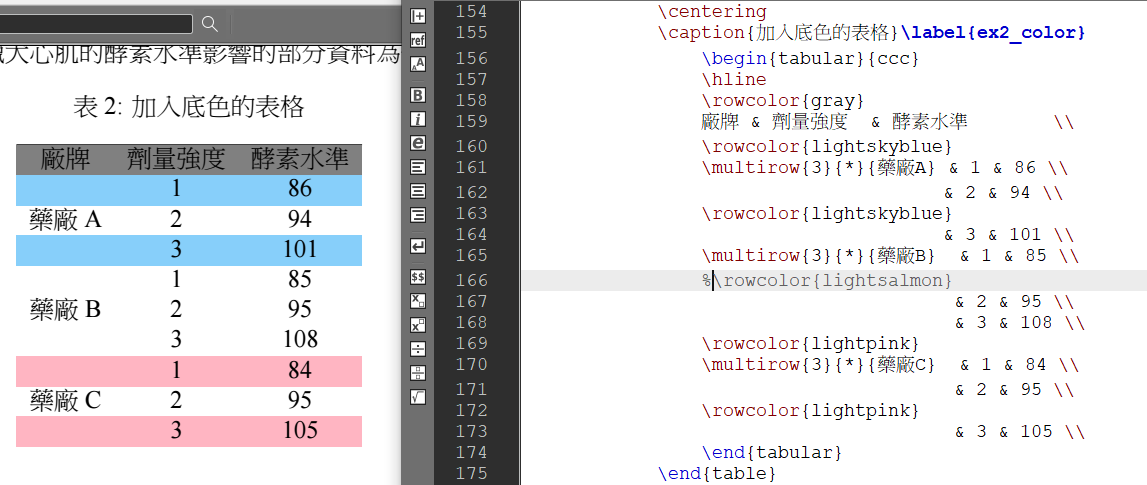
\includegraphics[scale=0.3]{q1_1.png}
		}
		\\
		\subfloat[單列著色後消失的列文字]{
		\label{q_rowcolor2}
		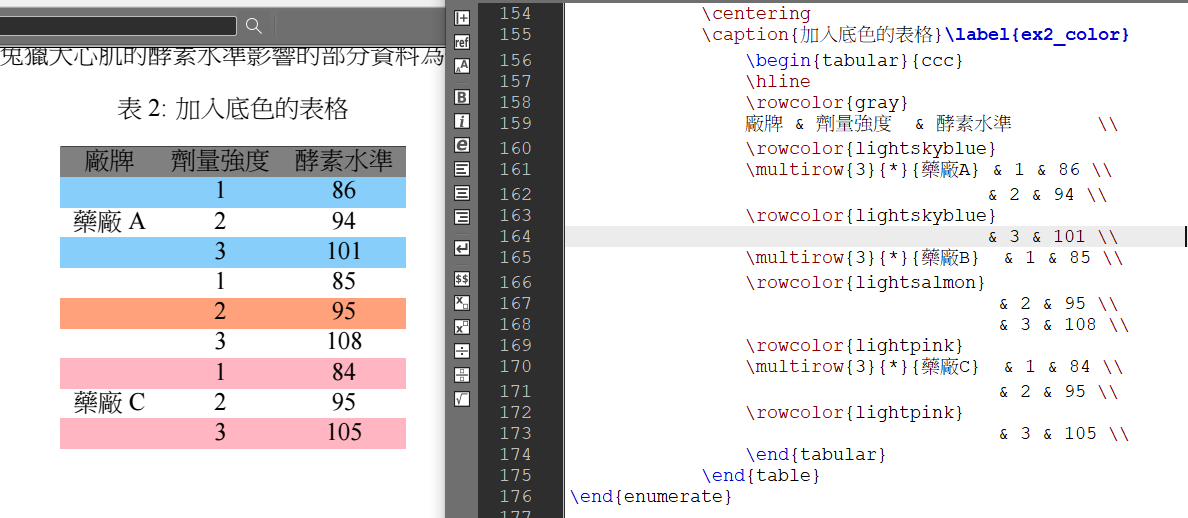
\includegraphics[scale=0.3]{q1_2.png}
		}
		\caption{跨列的單列著色問題} \label{q_rowcolor}
	\end{figure}

\newpage
\nocite{*}
\bibliographystyle{amsplain}
\bibliography{reference}


\end{document}